
\chapter{Design of a Multi-Trajectory Simulation Algorithm} 
\label{ch:Multi-Trajectory Simulation Algorithm}
This chapter introduces a design for a multi-trajectory simulation algorithm and provides explanations and examples of its main steps. The strength of this algorithm lies in its ability to run simulations within complex models, either with or without the presence of rare-events, and its adaptability to reach a wide coverage of the state space with efficiency in different types of models...

\section{Introduction to Multi-Trajectory}
\label{sec:Introduction to Multi-Trajectory}
Multi-trajectory simulation algorithm is based on particles, where a particle represents one possible trajectory of the simulation, and carries a weight that indicates the probability of that trajectory to happen. At any given time there is a collection of particles ready to be executed. Each particle is associated with one state of the model, and the execution of it implies a change in that state by following one or more of its possible transitions. 

The core idea of the algorithm can be described as a loop of three steps:
\begin{enumerate}
  \item Selection of the next particle...
  \item Execution of the particle, which consists in choosing between:
  \begin{enumerate}
    \item Move: Randomly select...
    \item Split: Create one new...
  \end{enumerate}
  \item Insertion of the particle...
\end{enumerate}


\begin{figure}[htb]
\begin{multicols}{3}
\centering
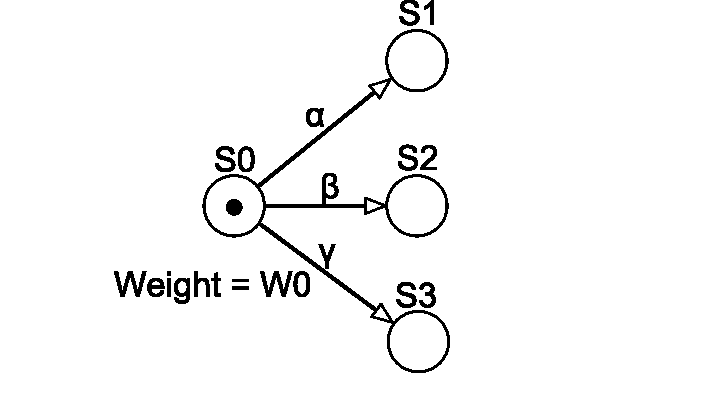
\includegraphics[width=.33\textwidth]{Model_Markov_Chain_Init.pdf}\\
Initial\\
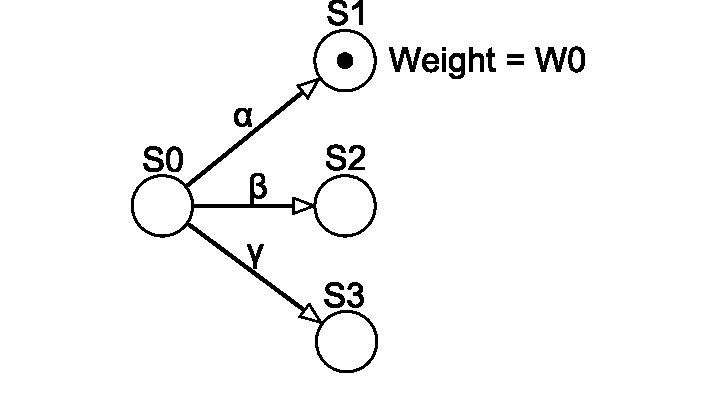
\includegraphics[width=.33\textwidth]{Model_Markov_Chain_Move.pdf}\\
Move, with probability $\alpha/(\alpha+\beta+\gamma)$\\
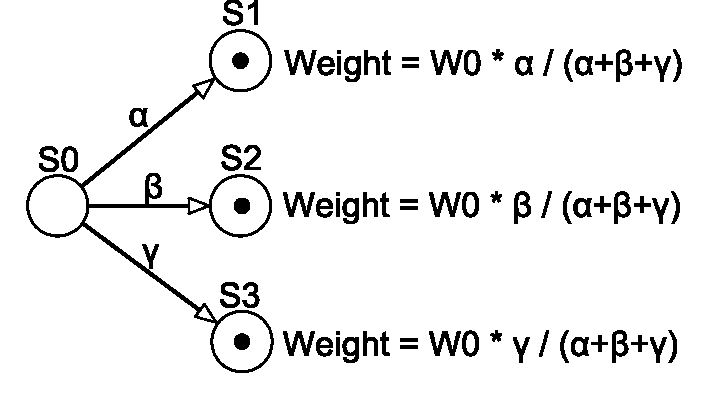
\includegraphics[width=.33\textwidth]{Model_Markov_Chain_Split.pdf}\\
Split\\
\end{multicols}
\caption{Move or Split Example}
\label{fig:Move or Split Example}
\end{figure}


Against expectations, after the implementation of these strategies the results obtained by the executions were incorrect. Different attempts were made to overcome this error without success. An analysis of it with a numerical example is presented in Section~\ref{sub:Markov Chain}. Due to this limitation a solution with a fair execution over the particles is chosen, using the definition of a cycle as the execution of all particles in the pool and the restriction of not execute a particle twice in a cycle.


\subsection*{Only Exponential Transitions Enabled}
If there are only exponential transitions enabled, ...  and the average time spent in the state is equal to the inverse of the sum of all those weighting factors.

\begin{flalign*}
\begin{array}{ccl}
Time\ Spent &=&\displaystyle\frac{\displaystyle 1}{\displaystyle\sum\limits_{i=0}^n (\frac{enabled_i}{delay_i})}\\
\\
Weighting\ Factor[i] &=&\left\lbrace 
	\begin{array}{ccl}
	Immediate\ Transition &=&0\\
	Exponential\ Transition &=&\displaystyle\frac{enabled_i}{delay_i}\\
	Deterministic\ Transition &=&0
	\end{array} 
\right.
\end{array}
\end{flalign*}

